% 2010 年上海卷文科第 20 题：圆柱形灯笼（无上底面，四个矩形骨架）。
% 来源 PDF：普通高考/2010/2010上海文.pdf，SHA-256 5e81bdb27659512a50968275bf502ee666e2ac3f25f9fcaa1b166576fbe9cf62。
% 原页：第 2 页（A3 三栏）第 1 栏上部，书页码 630。
% 重绘依据：按底面半径 r、高 h 的圆柱绘制，侧面四条等分竖线表示四个矩形骨架，不画上底面。
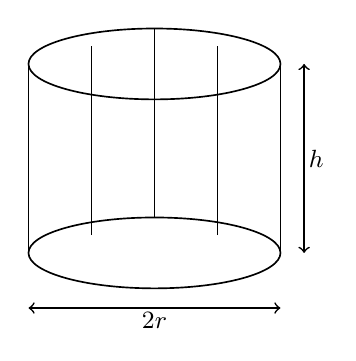
\begin{tikzpicture}[semithick, every node/.style={inner sep=1.4pt, font=\small}]
  % 下底椭圆
  \draw (0,0) ellipse (1.6 and 0.45);
  % 侧边
  \draw (-1.6,0) -- (-1.6,2.4);
  \draw (1.6,0) -- (1.6,2.4);
  % 上口（无上底面，只画椭圆口）
  \draw (0,2.4) ellipse (1.6 and 0.45);
  % 四条骨架竖线
  \draw (-1.6,0) -- (-1.6,2.4);
  \draw (-0.8,0.225) -- (-0.8,2.625);
  \draw (0,0.45) -- (0,2.85);
  \draw (0.8,0.225) -- (0.8,2.625);
  % 标注
  \draw[<->] (-1.6,-0.7) -- (1.6,-0.7);
  \node[below] at (0,-0.7) {$2r$};
  \draw[<->] (1.9,0) -- (1.9,2.4);
  \node[right] at (1.9,1.2) {$h$};
\end{tikzpicture}
